\begin{frame}{Punto de partida de la investigación}
\begin{block}{}
Consiste en hallar, formular problemas y luchar con ellos:
\begin{itemize}
    \item Criticar soluciones o problemas conocidos o existentes.
    \item Aplicar soluciones innovadoras a problemas conocidos o existentes o proponer soluciones conocidas a problemas innovadores.
    \item Buscar nuevas relaciones entre problemas ya conocidos.
    \item Abordar problemas ya conocidos desde distintos campos.
\end{itemize}
\end{block} 
\end{frame}
        
\begin{frame}{Elegir el tema de investigación}
\begin{block}{}
\begin{itemize}
    \item La elección se puede hacer buscando:
    \begin{itemize}
        \item Relevante:  Científico, social, tecnológico.
        \item Adecuado:  Para los empleados en la universidad, instituto y laboratorio de investigación.
    \end{itemize}
    \item Consultar tiempo y viabilidad para desarrollar la investigación. 
    \begin{itemize}
        \item Ámbito: No es necesario resolverlo todo. Es mejor limitarse luego ser demasiado amplio.
    \end{itemize}
\end{itemize}
\end{block} 
\end{frame}

\begin{frame}{Revisión bibliográfica}
\begin{block}{}
\begin{itemize}
    \item Está bien comenzar con libros y papers. Después de dominar las técnicas principales, busque trabajo relevante en buenos repositorios
    \item Puedes buscar exclusivamente en (Top Computer Science Conferences).
    \item Repositorios de busqueda:
    \begin{itemize}
        \item Scholar (http://scholar.google.com) 
        \item Scopus (http://www.scopus.com)
        \item  Web of Science (http://www.webofknowledge.com)
    \end{itemize}
\end{itemize}
\end{block}
\end{frame}

\begin{frame}{Planteamiento del problema}
\begin{block}{}
Es la explicación de tu tema o de lo que quieres hacer en tu trabajo, pero no funciona de esa manera. Se trata de establecer la problemática de tu investigación. 
\begin{itemize}
    \item ¿Eso qué quiere decir? Debes concretar una situación para analizarla, delimitarla, describirla y darle una posible solución o respuesta al por qué de sus causas o consecuencias.
\end{itemize}
\end{block}   
\end{frame}

\begin{frame}{Pregunta de investigación}
\begin{block}{}
 La pregunta principal de investigación es la pregunta que tu tesis pretende responder y deriva del planteamiento del problema que has formulado previamente. 
\end{block}   
\end{frame}

\begin{frame}{Hipótesis}
\begin{block}{}
\begin{itemize}
    \item  Es una posible solución al problema. quienes afirman que es un método de comprobación. [1]
    \item [--] Los buenos objetivos son impulsados por una buena hipótesis de investigación.
    \item [--] Definir una hipótesis sólida es lo que diferencia la investigación de un trabajo técnico.
\end{itemize}
\end{block} 
\end{frame}

\begin{frame}{Variables de la investigación}
\begin{block}{}
La clave para diseñar cualquier experimento o aplicaciones es ver qué variables de investigación podrían afectar el resultado. [1]
 \begin{itemize}
     \item Variable Independiente: Es el centro del experimento y desarrollada por el investigador.
     \item Variable Dependiente: Es el resultado medible de este desarrollo, los resultados experimentales o aplicaciones.
 \end{itemize}
\end{block}  
\end{frame}

\begin{frame}{Objetivos de la investigación}
\begin{block}{}
\begin{itemize}
    \item El objetivo se puede definir con una revisión tecnológica. [1]
    \item Debe ser una acción que solucione algún problema o problema existente.
    \item Debe ir acompañado de una hipótesis bien definida
\end{itemize}
\end{block}
 \begin{figure}[H]
    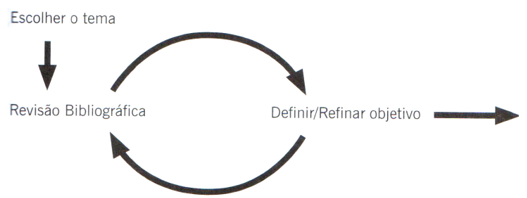
\includegraphics[scale=0.55]{images/figura4.PNG}
    \label{fig:boat1}
\end{figure}
\end{frame}

\begin{frame}{Evaluación}
\begin{block}{}
 \begin{itemize}
     \item ¿Cómo evaluar tu investigación?	
    \begin{itemize}
        \item Defina, lo antes posible, cómo medir sus resultados para entender qué tan cerca está del objetivo principal.
        \begin{itemize}
            \item Me esfuerzo mucho, pero si es necesario, suelta / cambia la idea inicial.
        \end{itemize}
    \end{itemize}
    \item Dado que generalmente el 90\% de los resultados son realmente fallos, debemos asegurarnos de que estamos evaluando correctamente los resultados, desde el principio
    \begin{itemize}
        \item Comprender que toda investigación tiene limitaciones y puntos débiles.
    \end{itemize}
 \end{itemize}  
 \end{block}
\end{frame}

\begin{frame}{Implementación}
\begin{block}{}
\begin{itemize}
    \item Puedo ser innovador o no.
    \item Si falta una hipótesis, entonces no es así.
    \item Cuando es innovador, suele ser explorador.
    \item Si se trata de un sistema o reproducción, puede informarse en un “Informe técnico”.
    \item Aceptable para proyectos finales de pregrado (TCC), pero difícilmente para maestrías o doctorados
\end{itemize}
\end{block}
\end{frame}

